\documentclass{article}
\usepackage[utf8]{inputenc} % Handle UTF-8 encoding
\usepackage{amsmath, amssymb, tikz, geometry, multicol}
\usetikzlibrary{calc}
\geometry{margin=0.15in}
\tolerance=1000

\begin{document}

% Start of the document with two columns
\begin{multicols}{2}

% Left Column: Triangles
\section*{Trigonometry with Triangles}

\subsection*{Right Triangle Definitions}
\begin{center}
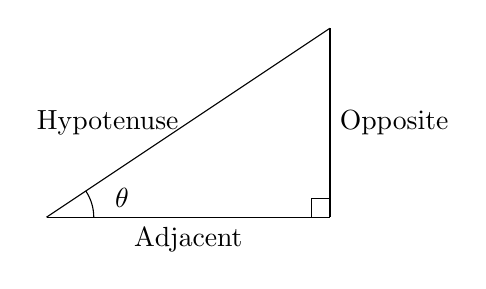
\begin{tikzpicture}[scale=1.2]
    \coordinate (A) at (0,0);
    \coordinate (B) at (3,0);
    \coordinate (C) at (3,2);
    \draw (A) -- node[below] {Adjacent} (B);
    \draw (A) -- node[left] {Hypotenuse} (C);
    \draw (B) -- node[right] {Opposite} (C);
    \draw (A) ++(0.5,0) arc (0:33.69:0.5cm);
    \node at (0.8,0.2) {\(\theta\)};
    % Right angle symbol
    \draw (B) ++(-0.2,0) -- ++(0,0.2) -- ++(0.2,0);
\end{tikzpicture}
\end{center}
\[
\sin \theta = \dfrac{\text{Opposite}}{\text{Hypotenuse}}, \quad
\cos \theta = \dfrac{\text{Adjacent}}{\text{Hypotenuse}}, \quad
\tan \theta = \dfrac{\text{Opposite}}{\text{Adjacent}}
\]
\[
\tan \theta = \dfrac{\sin \theta}{\cos \theta}, \quad
\csc \theta = \dfrac{1}{\sin \theta}, \quad
\sec \theta = \dfrac{1}{\cos \theta}, \quad
\cot \theta = \dfrac{1}{\tan \theta}
\]

\subsection*{Reference Angles}

A reference angle is the acute angle (\(<90^\circ\)) formed by the terminal side of an angle and the horizontal axis.

\begin{center}
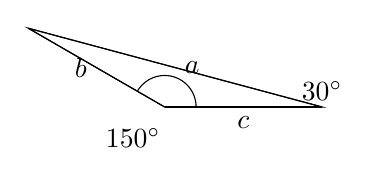
\begin{tikzpicture}[scale=2]
    % Define points
    \coordinate (A) at (0,0); % Point A (origin)
    \coordinate (B) at (1,0); % Point B on the positive x-axis
    % Point C calculated to form a 150-degree angle at A
    \coordinate (C) at ({cos(150)}, {sin(150)}); % Coordinates using degrees

    % Draw triangle
    \draw (A) -- (B) -- (C) -- cycle;

    % Label sides
    \draw (A) -- node[below]{$c$} (B);
    \draw (B) -- node[right]{$a$} (C);
    \draw (C) -- node[left]{$b$} (A);

    % Mark angle at A (150 degrees)
    \draw (A) ++(0.2,0) arc (0:150:0.2cm);

    % Move the 150-degree label outside the triangle towards the bottom left
    \node at ($(A)+(-0.2,-0.2)$) {\(150^\circ\)};

    \node at ($(A)+(1,0.1)$) {\(30^\circ\)};
\end{tikzpicture}
\end{center}

In this triangle, angle \( A \) is \(150^\circ\), and the reference angle \( \theta_{\text{ref}} \) is:

\[
\theta_{\text{ref}} = 180^\circ - 150^\circ = 30^\circ
\]

\textbf{Example:} Find the reference angle for \( \theta = 150^\circ \).

\[
\theta_{\text{ref}} = 180^\circ - 150^\circ = 30^\circ
\]

So, the reference angle is \(30^\circ\).

When calculating trigonometric functions for obtuse angles, use the reference angle and adjust the sign based on the quadrant.

\textbf{Example:} Find \(\sin 150^\circ\).

\[
\sin 150^\circ = \sin (180^\circ - 30^\circ) = \sin 30^\circ = \dfrac{1}{2}
\]

Since \(150^\circ\) is in Quadrant II, (sin+), \(\sin 150^\circ = \dfrac{1}{2}\).

\subsection*{Signs of Trigonometric Functions}
\begin{center}
\begin{tabular}{|c|c|}
\hline
Quadrant & Positive Functions \\
\hline
I & \(\sin\), \(\cos\), \(\tan\) \\
II & \(\sin\) \\
III & \(\tan\) \\
IV & \(\cos\) \\
\hline
\end{tabular}
\end{center}

\subsection*{Inverse Functions}
\noindent
The range of \(\theta = \arccos(x)\) is given by \(0 \leq \theta \leq \pi\).

\noindent
The range of \(\theta = \arcsin(x)\) is given by \(-\frac{\pi}{2} \leq \theta \leq \frac{\pi}{2}\).

\noindent
The range of \(\theta = \arctan(x)\) is given by \(-\frac{\pi}{2} < \theta < \frac{\pi}{2}\).

\subsection*{Pythagorean Identity}
\[
\sin^2 \theta + \cos^2 \theta = 1
\]
\textbf{Example:} If \( \sin \theta = \dfrac{3}{5} \), then:
\[
\cos \theta = \sqrt{1 - \left( \dfrac{3}{5} \right)^2} = \dfrac{4}{5}
\]
\subsection*{Sum and Difference Formulas for Sine \emph{and} Cosine}

\[
\sin(x + y) \;=\; \sin x \cos y \;+\; \cos x \sin y,
\]
\[
\sin(x - y) \;=\; \sin x \cos y \;-\; \cos x \sin y,
\]

\[
\cos(x + y) \;=\; \cos x \cos y \;-\; \sin x \sin y,
\]
\[
\cos(x - y) \;=\; \cos x \cos y \;+\; \sin x \sin y.
\]

These identities allow us to break down more complicated trigonometric expressions into simpler combinations of sines and cosines of single angles.  

\textbf{Example (using cosine):} Find \(\cos(75^\circ)\) using the sum formula.  

Since \(75^\circ = 45^\circ + 30^\circ\), we write:

\[
\cos(75^\circ) \;=\; \cos\bigl(45^\circ + 30^\circ\bigr).
\]

Using the sum formula for cosine:

\[
\cos(45^\circ + 30^\circ)
\;=\;
\cos 45^\circ \,\cos 30^\circ \;-\; \sin 45^\circ \,\sin 30^\circ.
\]

Substitute known values:
\[
\cos 45^\circ = \frac{\sqrt{2}}{2}, 
\quad
\sin 45^\circ = \frac{\sqrt{2}}{2},
\quad
\cos 30^\circ = \frac{\sqrt{3}}{2}, 
\quad
\sin 30^\circ = \frac{1}{2}.
\]

\[
\cos(75^\circ)
= \left(\frac{\sqrt{2}}{2}\right)\!\left(\frac{\sqrt{3}}{2}\right)
- \left(\frac{\sqrt{2}}{2}\right)\!\left(\frac{1}{2}\right).
\]

\[
\cos(75^\circ)
= \frac{\sqrt{6}}{4} \;-\; \frac{\sqrt{2}}{4}
= \frac{\sqrt{6} - \sqrt{2}}{4}.
\]

Hence,
\[
\boxed{\cos(75^\circ) = \frac{\sqrt{6} - \sqrt{2}}{4}.}
\]

These sum and difference formulas are fundamental tools in trigonometry for simplifying expressions, evaluating trigonometric functions at specific angles, and deriving many other identities.

\subsection*{Sum of Sine and Cosine in Amplitude-Phase Form}

A common problem in trigonometry is to rewrite a linear combination of sine and cosine,
\[
a \sin x \;+\; b \cos x,
\]
in \emph{amplitude-phase form} (also called \emph{phase-shift form}), which typically looks like
\[
R \sin\!\bigl(x + \phi\bigr),
\]
or sometimes
\[
R \cos\!\bigl(x - \phi\bigr).
\]

\subsubsection*{Key Steps}

\begin{enumerate}
\item \textbf{Identify the coefficients:}
  \[
  a \sin x + b \cos x.
  \]
\item \textbf{Compute the amplitude \(R\):}  
  We define
  \[
    R = \sqrt{\,a^2 + b^2\,}.
  \]
  This follows from the Pythagorean identity once you set up the system:
  \[
    \begin{cases}
      R \cos \phi = a,\\[6pt]
      R \sin \phi = b.
    \end{cases}
  \]
  Squaring and adding both equations gives
  \[
    (R \cos \phi)^2 + (R \sin \phi)^2 \;=\; a^2 + b^2,
  \]
  and using \(\cos^2 \phi + \sin^2 \phi = 1\) leads to
  \[
    R^2 = a^2 + b^2.
  \]
\item \textbf{Solve for the phase \(\phi\):}
  From the system
  \[
    \begin{cases}
      R \cos \phi = a,\\[6pt]
      R \sin \phi = b,
    \end{cases}
  \]
  you can divide one equation by the other to get
  \[
    \tan \phi = \dfrac{b}{a}
    \quad(\text{assuming }a \neq 0).
  \]
  Then
  \[
    \phi = \arctan\!\Bigl(\dfrac{b}{a}\Bigr),
  \]
  with possible adjustments depending on the signs of \(a\) and \(b\) (to get \(\phi\) in the correct quadrant).
\item \textbf{Rewrite in the new form:}
  Once \(R\) and \(\phi\) are found, you have:
  \[
    a \sin x + b \cos x = R \sin\bigl(x + \phi\bigr).
  \]
  This identity can be verified using the sum formula for sine:
  \[
    R \sin(x + \phi) = R\bigl[\sin x \cos \phi + \cos x \sin \phi\bigr]
    = R \cos \phi\, \sin x + R \sin \phi\, \cos x,
  \]
  and noting that \(R \cos \phi = a\) and \(R \sin \phi = b\).
\end{enumerate}

\subsubsection*{Example}

Rewrite \(3 \sin x + \sqrt{3}\,\cos x\) in amplitude-phase form:

\begin{enumerate}
\item Identify \(a = 3\) and \(b = \sqrt{3}\).
\item Compute the amplitude:
  \[
    R = \sqrt{\,a^2 + b^2\,}
      = \sqrt{\,3^2 + (\sqrt{3})^2\,}
      = \sqrt{9 + 3}
      = \sqrt{12}
      = 2\sqrt{3}.
  \]
\item Solve for \(\phi\).  We want:
  \[
    2\sqrt{3}\,\cos \phi = 3
    \quad\Longrightarrow\quad
    \cos \phi = \frac{3}{2\sqrt{3}} = \frac{\sqrt{3}}{2},
  \]
  \[
    2\sqrt{3}\,\sin \phi = \sqrt{3}
    \quad\Longrightarrow\quad
    \sin \phi = \frac{\sqrt{3}}{2\sqrt{3}} = \frac{1}{2}.
  \]
  These correspond to \(\phi = \tfrac{\pi}{6}\) (since \(\cos \tfrac{\pi}{6} = \sqrt{3}/2\) and \(\sin \tfrac{\pi}{6} = 1/2\)).
\item Write the final expression:
  \[
    3 \sin x + \sqrt{3}\,\cos x
    = 2\sqrt{3}\,\sin\!\Bigl(x + \tfrac{\pi}{6}\Bigr).
  \]
\end{enumerate}

This method works in general for any linear combination \(a \sin x + b \cos x\) and is especially helpful for analyzing maxima, minima, and phase shifts of trigonometric functions.

\subsection*{Double Angle Formulas}
\[
\sin(2\theta) = 2\sin(\theta)\cos(\theta)
\]
\[
\cos(2\theta) = \cos^2(\theta) - \sin^2(\theta),
\]

and using the Pythagorean identity \(\sin^2(\theta) + \cos^2(\theta) = 1\), we can derive alternate forms:

1. Replace \(\sin^2(\theta)\) with \(1 - \cos^2(\theta)\):
\[
\cos(2\theta) = \cos^2(\theta) - (1 - \cos^2(\theta)) = 2\cos^2(\theta)-1.
\]

2. Replace \(\cos^2(\theta)\) with \(1 - \sin^2(\theta)\):
\[
\cos(2\theta) = (1 - \sin^2(\theta)) - \sin^2(\theta) = 1 - 2\sin^2(\theta).
\]

Thus, the double angle formula for cosine can be expressed in three equivalent ways:
\[
\cos(2\theta) = \cos^2(\theta) - \sin^2(\theta) = 2\cos^2(\theta)-1 = 1-2\sin^2(\theta).
\]

\subsection*{Law of Sines}
\begin{center}
\begin{tikzpicture}[scale=1.2]
    \coordinate (A) at (0,0);
    \coordinate (B) at (3,0);
    \coordinate (C) at (1.5,2.5);
    \draw (A) -- node[below] {$c$} (B) -- node[right] {$a$} (C) -- node[left] {$b$} (A);
    \node[below left] at (A) {$A$};
    \node[below right] at (B) {$B$};
    \node[above] at (C) {$C$};
\end{tikzpicture}
\end{center}
\[
\frac{\sin A}{a} = \frac{\sin B}{b} = \frac{\sin C}{c}
\]
\textbf{Example:} If \( a = 7 \), \( A = 30^\circ \), and \( B = 45^\circ \), find \( b \):
\begin{align*}
\frac{a}{\sin A} &= \frac{b}{\sin B} \\
b &= a \times \frac{\sin B}{\sin A} \\
&= 7 \times \frac{\sin 45^\circ}{\sin 30^\circ} \\
&= 7 \times \frac{\frac{\sqrt{2}}{2}}{\frac{1}{2}} \\
&= 7 \times \sqrt{2} \approx 9.9
\end{align*}

\subsection*{Law of Cosines}
\[
a^2 = b^2 + c^2 - 2bc \cos A
\]
\textbf{Example:} Given \( b = 5 \), \( c = 7 \), and \( A = 60^\circ \):
\begin{align*}
a^2 &= 5^2 + 7^2 - 2 \times 5 \times 7 \times \cos 60^\circ \\
&= 25 + 49 - 70 \times \left( \dfrac{1}{2} \right) \\
&= 74 - 35 \\
&= 39 \\
a &= \sqrt{39} \approx 6.24
\end{align*}

\subsection*{Area of a Triangle}
\[
\text{Area} = \dfrac{1}{2} ab \sin C
\]
\textbf{Example:} For \( a = 5 \), \( b = 7 \), and \( C = 45^\circ \):
\[
\text{Area} = \dfrac{1}{2} \times 5 \times 7 \times \sin 45^\circ = \dfrac{35}{2} \times \dfrac{\sqrt{2}}{2} = \dfrac{35\sqrt{2}}{4} \approx 12.37
\]

\end{multicols}

% Start a new page and begin a new multicolumn environment
\newpage
\begin{multicols}{2}

% Right Column: Circles
\section*{Unit Circle and Angles}

\subsection*{Unit Circle Diagram}
\begin{center}
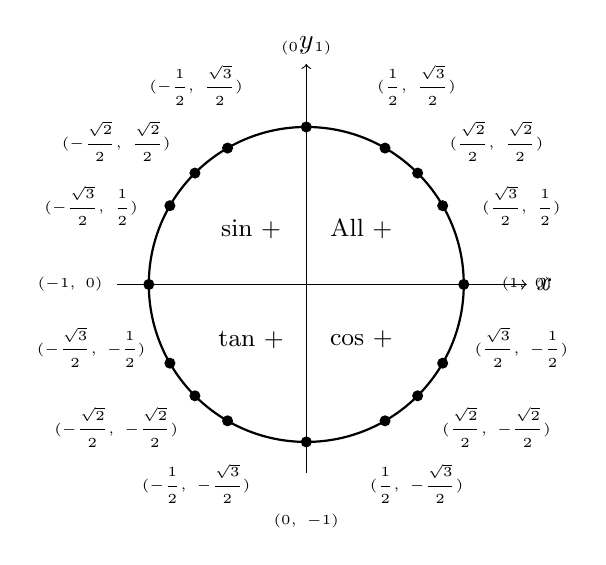
\begin{tikzpicture}[scale=2]
    % Draw the unit circle
    \draw[thick] (0,0) circle (1cm);
    % Axes
    \draw[->] (-1.2,0) -- (1.4,0);
    \draw[->] (0,-1.2) -- (0,1.4);
    % x and y labels adjusted
    \node[right] at (1.4,0) {$x$};
    \node[above] at (0,1.4) {$y$};
    % Points at common angles with labels
    \foreach \a/\d/\cs/\sn/\dx/\dy in {
        0/0^\circ/1/0/0.4/0.0,
        30/30^\circ/\dfrac{\sqrt{3}}{2}/\dfrac{1}{2}/0.5/0,
        45/45^\circ/\dfrac{\sqrt{2}}{2}/\dfrac{\sqrt{2}}{2}/0.5/0.2,
        60/60^\circ/\dfrac{1}{2}/\dfrac{\sqrt{3}}{2}/0.2/0.4,
        90/90^\circ/0/1/0.0/0.5,
        120/120^\circ/-\dfrac{1}{2}/\dfrac{\sqrt{3}}{2}/-0.2/0.4,
        135/135^\circ/-\dfrac{\sqrt{2}}{2}/\dfrac{\sqrt{2}}{2}/-0.5/0.2,
        150/150^\circ/-\dfrac{\sqrt{3}}{2}/\dfrac{1}{2}/-0.5/0,
        180/180^\circ/-1/0/-0.5/0.0,
        210/210^\circ/-\dfrac{\sqrt{3}}{2}/-\dfrac{1}{2}/-0.5/0.1,
        225/225^\circ/-\dfrac{\sqrt{2}}{2}/-\dfrac{\sqrt{2}}{2}/-0.5/-0.2,
        240/240^\circ/-\dfrac{1}{2}/-\dfrac{\sqrt{3}}{2}/-0.2/-0.4,
        270/270^\circ/0/-1/0.0/-0.5,
        300/300^\circ/\dfrac{1}{2}/-\dfrac{\sqrt{3}}{2}/0.2/-0.4,
        315/315^\circ/\dfrac{\sqrt{2}}{2}/-\dfrac{\sqrt{2}}{2}/0.5/-0.2,
        330/330^\circ/\dfrac{\sqrt{3}}{2}/-\dfrac{1}{2}/0.5/0.1
    } {
        % Calculate coordinates
        \coordinate (P) at ({cos(\a)},{sin(\a)});
        % Draw point
        \fill (P) circle (1pt);
        % Label coordinates
        \node[font=\tiny, anchor=center] at ($(P)+(\dx,\dy)$) {$(\cs,\ \sn)$};
    }
    % Quadrants
    \node at (0.35,0.35) {\small All $+$};
    \node at (-0.35,0.35) {\small $\sin$ $+$};
    \node at (-0.35,-0.35) {\small $\tan$ $+$};
    \node at (0.35,-0.35) {\small $\cos$ $+$};
\end{tikzpicture}
\end{center}
The cosine is the x-value, the sine is the y-value.

\subsection*{Radians and Degrees}
\[
180^\circ = \pi \text{ radians}, \quad 1^\circ = \dfrac{\pi}{180} \text{ radians}
\]
\textbf{Example:} Convert \( 135^\circ \) to radians:
\[
135^\circ \times \dfrac{\pi}{180^\circ} = \dfrac{3\pi}{4}
\]

\subsection*{Alternate Formulation}
For common angles, sine and cosine values can be calculated as:
\[
\sin \theta = \dfrac{\sqrt{n}}{2}, \quad \cos \theta = \dfrac{\sqrt{4 - n}}{2}
\]
where \( n \) corresponds to the following angles:
\begin{center}
\begin{tabular}{ll}
\( n = 0 \) & for \( \theta = 0^\circ \), \\
\( n = 1 \) & for \( \theta = 30^\circ \), \\
\( n = 2 \) & for \( \theta = 45^\circ \), \\
\( n = 3 \) & for \( \theta = 60^\circ \), \\
\( n = 4 \) & for \( \theta = 90^\circ \). \\
\end{tabular}
\end{center}

\subsection*{Reference Angles on the Unit Circle}
To find the trigonometric functions of any angle, find its reference angle and determine the sign based on the quadrant.

\textbf{Example:} Find \(\tan 225^\circ\).
\[
\theta_{\text{ref}} = 225^\circ - 180^\circ = 45^\circ
\]
\[
\tan 225^\circ = \tan (180^\circ + 45^\circ) = \tan 45^\circ = 1
\]
Since \(225^\circ\) is in Quadrant III, \(\tan\) is positive.

\textbf{Example:} Find \(\sin 210^\circ\).
\[
\theta_{\text{ref}} = 210^\circ - 180^\circ = 30^\circ
\]
\[
\sin 210^\circ = -\sin 30^\circ = -\dfrac{1}{2}
\]
Since \(210^\circ\) is in Quadrant III, \(\sin\) is negative.

\textbf{Example:} Find \(\cos 300^\circ\).
\[
\theta_{\text{ref}} = 360^\circ - 300^\circ = 60^\circ
\]
\[
\cos 300^\circ = \cos (360^\circ - 60^\circ) = \cos 60^\circ = \dfrac{1}{2}
\]
Since \(300^\circ\) is in Quadrant IV, \(\cos\) is positive.

\subsection*{Coterminal Angles}
Angles that differ by full rotations (\(360^\circ\)) are coterminal.

\textbf{Example:} \( \theta = -30^\circ \) is coterminal with \( 330^\circ \) because:
\[
-30^\circ + 360^\circ = 330^\circ
\]

\subsection*{Period of Stretched Trigonometric Functions}

For trigonometric functions that are stretched or compressed horizontally, the period changes accordingly.

- For functions with a natural period of \( 2\pi \) (such as \( \sin x \) and \( \cos x \)):

\[
T = \dfrac{2\pi}{B}
\]

- For functions with a natural period of \( \pi \) (such as \( \tan x \) and \( \cot x \)):

\[
T = \dfrac{\pi}{B}
\]

Where \( B \) is the coefficient of \( x \) in the function \( f(x) = \sin(Bx) \) or \( f(x) = \tan(Bx) \).

\textbf{Example:} Find the period of \( f(x) = \sin(2x) \).

Since the natural period of \( \sin x \) is \( 2\pi \):

\[
T = \dfrac{2\pi}{B} = \dfrac{2\pi}{2} = \pi
\]

So, the period of \( \sin(2x) \) is \( \pi \).

\textbf{Example:} Find the period of \( f(x) = \tan\left( \dfrac{x}{3} \right) \).

Since the natural period of \( \tan x \) is \( \pi \):

\[
T = \dfrac{\pi}{B} = \dfrac{\pi}{\dfrac{1}{3}} = 3\pi
\]

So, the period of \( \tan\left( \dfrac{x}{3} \right) \) is \( 3\pi \).

\end{multicols}

\end{document}
